\section{Órbita inicial}
\label{sec_fases_orbita_inicial}

Assume-se neste trabalho que o lançador realiza a inserção da espaçonave perseguidora em uma órbita circular de $500$~km de altitude (raio orbital de $6.878,137$~km) coplanar à órbita da espaçonave alvo. 

A altitude escolhida situa-se na faixa da Óribta de Baixa Altitude (\gls{leo}), região onde diversas missões de encontro e acoplamento orbital são conduzidas. 
Como referência, a \gls{iss} opera aproximadamente entre $370$ e $460$~km de altitude \cite{ISSaltitude}. 
A adoção de uma altitude de $500$~km reduz os efeitos de arrasto atmosférico em comparação com órbitas mais baixas, ainda mais que o tempo de simulação é curto, um pouco mais que $2$ horas.

Com a inserção orbital realizada, o perseguidor passa a propagar seu movimento em uma órbita circular próxima à do alvo. 
A partir dessa configuração inicial, tornam-se possíveis as manobras de redução da diferença de fase orbital e em sequência, a transferência orbital, aqui chamada de aproximação de longa distância.

A Figura~\ref{fig_injecao_orbita_inicial} ilustra a configuração relativa das espaçonaves imediatamente após a injeção orbital do perseguidor.

\begin{figure}[H]
\centering
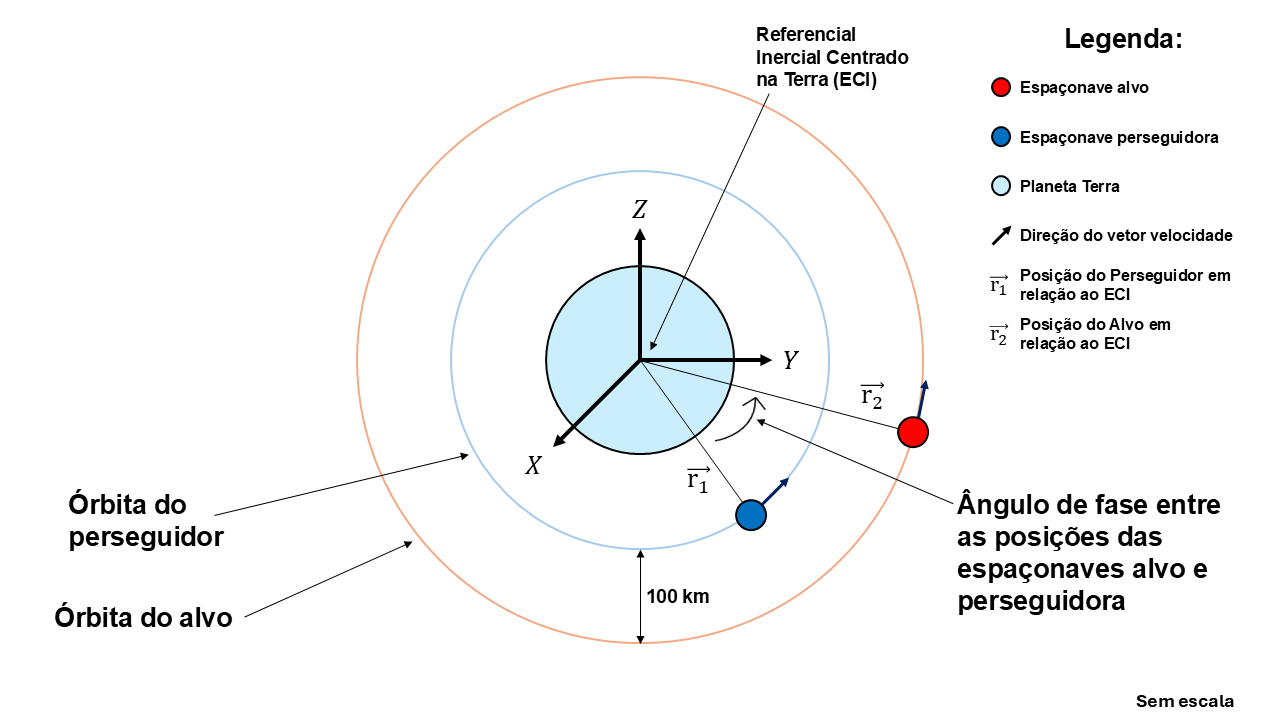
\includegraphics[width=1\linewidth]{3 Procedimento simulacao/Imagens/1 Posicao espaconaves injecao orbital.png}
\caption{Configuração relativa entre a espaçonave perseguidora e a espaçonave alvo após a inserção orbital do perseguidor.}
\label{fig_injecao_orbita_inicial}
\end{figure}

Após essa etapa inicial, inicia-se a fase de aproximação de longa distância, na qual o movimento do perseguidor é descrito no referencial inercial.